\clearpage

\lehead[]{\normalfont\sffamily\hspace*{-2.00cm}\textcolor{white}{\colorbox{lightblue}{\parbox[c][0.70cm][b]{1.60cm}{
\makebox[1.60cm][r]{\thechapter}\\ \makebox[1.60cm][r]{ÜBUNG}}}}\hspace{0.17cm}\textcolor{lightblue}{\chaptertitle}}
\rohead[]{\textcolor{lightblue}{\chaptertitle}\normalfont\sffamily\hspace*{0.17cm}\textcolor{white}{\colorbox{lightblue}{\parbox[c][0.70cm][b]{1.60cm}{\thechapter\\
ÜBUNG}}}\hspace{-2.00cm}}
%\chead[]{}
\rehead[]{\textcolor{lightblue}{AvHG, Inf, My}}
\lohead[]{\textcolor{lightblue}{AvHG, Inf, My}}

\section{ER-Modell -- Übung}

\subsection{Aufgabe 1: Interpretation eines ER-Diagramms}

\begin{compactenum}[a)]
\item Interpretiere das folgende Entity-Relationship-Diagramm:

\vspace{2mm}
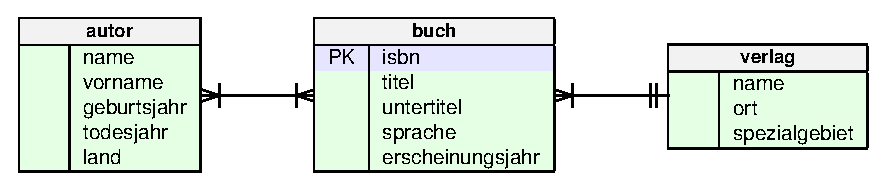
\includegraphics[width=0.80\textwidth]{./inf/SEKII/34_SQL_ER-Diagramme/ermAufgabe1.eps}
\vspace{2mm}

Achtung: Das abgebildete ER-Diagramm ist unvollständig. Es fehlen -- unter
anderem -- einige Schlüsselfelder! Welche?

Vervollständige das ER-Diagramm!

\vspace{1mm}

\item Erstelle ein SQL-Skript \myUserInput{buecherei.sql}, mit dem diese
Datenbank erzeugt werden kann.
\end{compactenum}


\subsection{Aufgabe 2: Kardinalitäten}

Welche Art von Beziehung besteht zwischen folgenden Entitätstypen? 

\emph{Achtung}: Entitätstyp (also Tabelle) bedeutet natürlich auch, dass es
jeweils mehrere Entitäten (Datensätze) gibt! Von jeweils beiden genannten Entitätstypen
\ldots

\begin{compactenum}[a)]
\item Mann, Frau (Beziehung: „verheiratet“)
\item Lehrer, Schüler
\item Esstisch, Stuhl
\item Tutor, Tutand
\item Schauspieler, Kinofilm (Beziehung: „spielen in“)
\end{compactenum}


\subsection{Aufgabe 3: Datenbankentwurf}

\begin{compactenum}[a)] 
\item Entwirf ein ER-Diagramm für einen Video-Verleih:\\
Für die Videos sollen der Titel, der Regisseur, das Erscheinungsjahr und eine
Identifikationsnummer abgespeichert werden. Für jeden Kunden wird die
vollständige Adresse abgespeichert. Ein Video darf maximal zwei Wochen
ausgeliehen werden. Danach ist eine einmalige Verlängerung um weitere zwei
Wochen möglich. Es ist wichtig, dass die Informationen über die Ausleihe nach
Rückgabe eines Videos nicht gelöscht werden, damit man im Nachhinein überprüfen
kann, wer wann welches Video ausgeliehen hatte.
\item Erstelle ein SQL-Skript \myFile{videothek.sql}, mit dem diese
Datenbank erzeugt werden kann.
\end{compactenum}

\pagebreak
 
\subsection{Aufgabe 4: Vergleich mit UML}

Vergleiche das Entity-Relationship-Modell mit dem Modell objektorientierter
Programmiersprachen, die man mit UML-Diagrammen entwirft.


\begin{compactenum}[a)]
\item Setze die Begriffe aus UML mit dem ER-Modell in Beziehung:

\vspace{2mm}

\bgroup
\def\arraystretch{1.2}
\begin{tabular}{|l|l|}\hline
\textbf{Begriff in UML} & \textbf{Entsprechender Begriff im ER-Modell\hspace{2cm}}
\\
\hline Klasse & \\ \hline
Objekt & \\ \hline
Attribut & \\ \hline
Methode & \\ \hline
(normale) Beziehung & \\ \hline
Aggregations-Beziehung & \\ \hline
Vererbungs-Beziehung & \\ \hline
\end{tabular}
\egroup

\vspace{2mm}

\item Was sind die wesentlichsten Unterschiede zwischen dem ER-Modell und dem
UML-Modell?
\end{compactenum}
